\chapter{Apoio à Docência} % (fold)
\label{chap:Apoio à Docência}
Neste capítulo, apresentaremos os principais recursos físicos e estruturais da \ac{GPF}, disponíveis aos docentes para melhor desempenharem suas atividades.

\section{Sala dos Professores} % (fold)
\label{sec:Sala dos Professores}
\setlength\intextsep{0pt}
\begin{wrapfigure}[9]{r}{0.5\textwidth}
	\centering
	\caption{Sala dos Professores}
	\label{fig:sala-prof}
	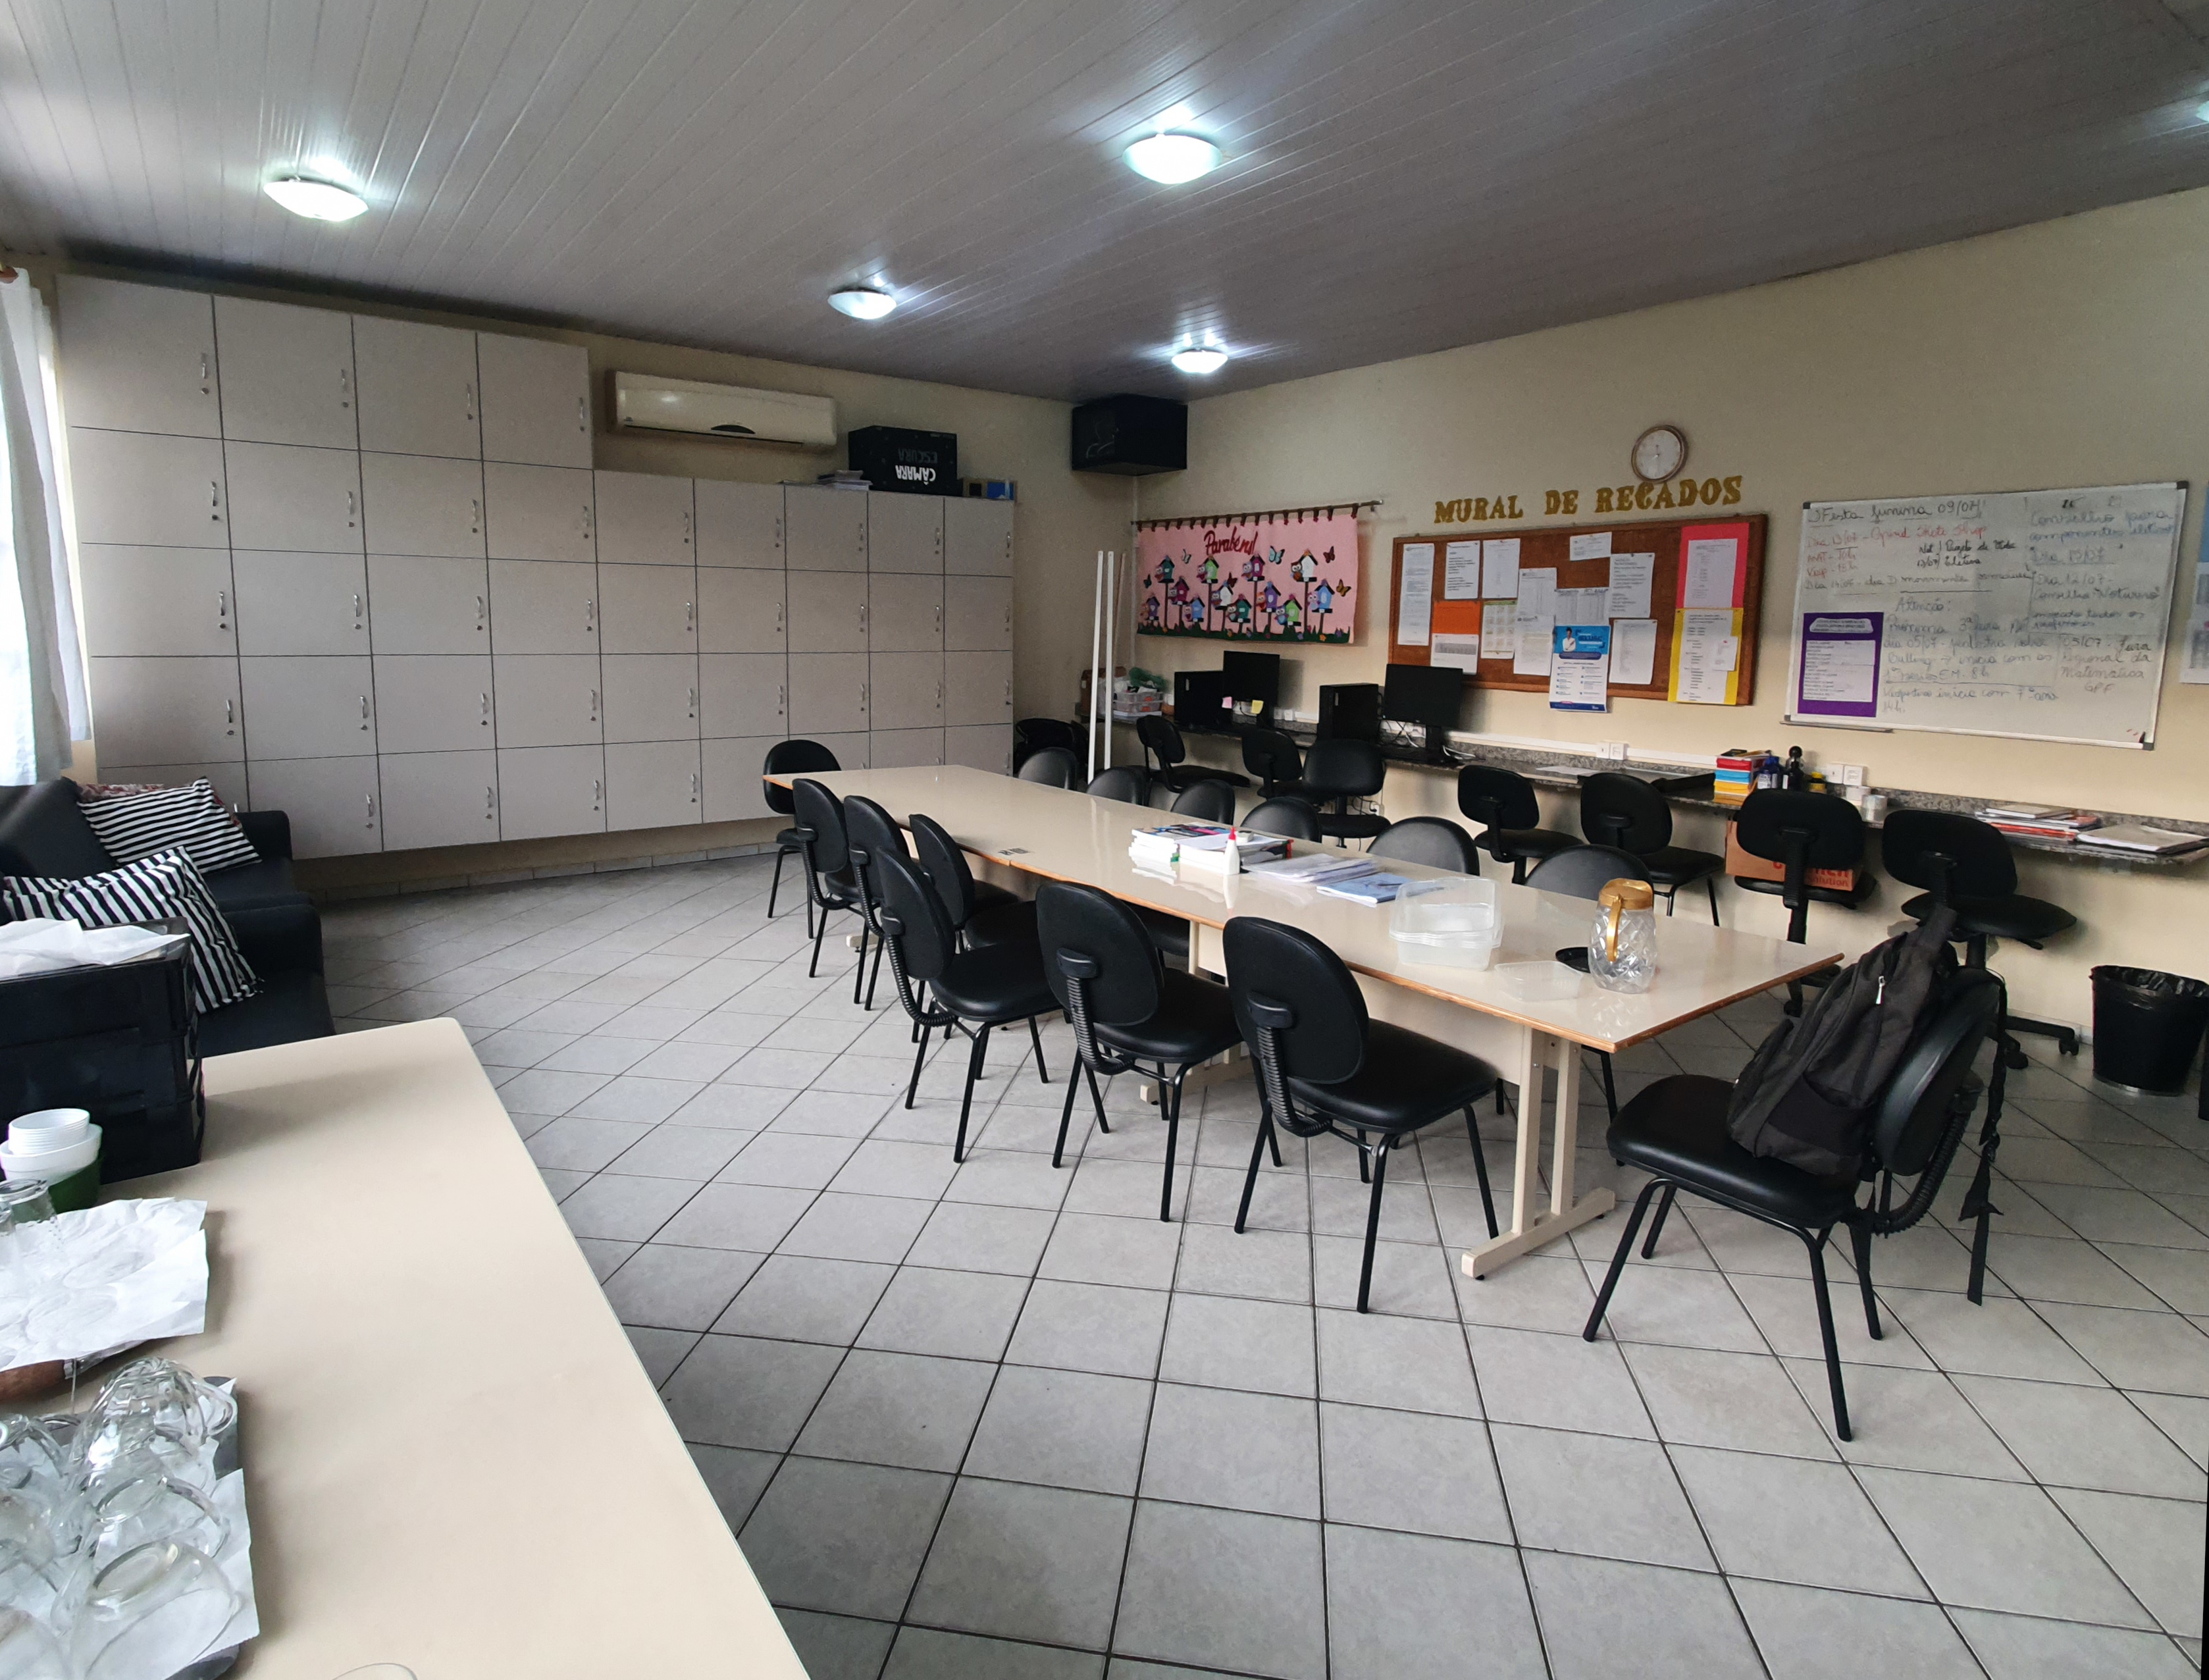
\includegraphics[width=.45\textwidth]{assets/sala-prof.jpg}
	\legend{Fonte: O autor}
\end{wrapfigure}
A Sala dos Professores, \autoref{fig:sala-prof}, possui: geladeira, forno de micro-ondas, aparelho de ar-condicionado e um purificador de água. É equipada com dois desktops conectados à internet. Cada professor tem um espaço nos armários nele os docentes geralmente guardam seus pertences pessoais ou recursos de aulas quaisquer que sejam e que necessitem de algum cuidado no manuseio. 
% section Sala dos Professores (end)

\section{Sala de Aula} % (fold)
\label{sec:Sala de Aula}
\setlength\intextsep{0pt}
\begin{wrapfigure}[12]{l}{0.5\textwidth}
	\centering
	\caption{Imagem da Lousa Digital}
	\label{fig:d-lousa}
	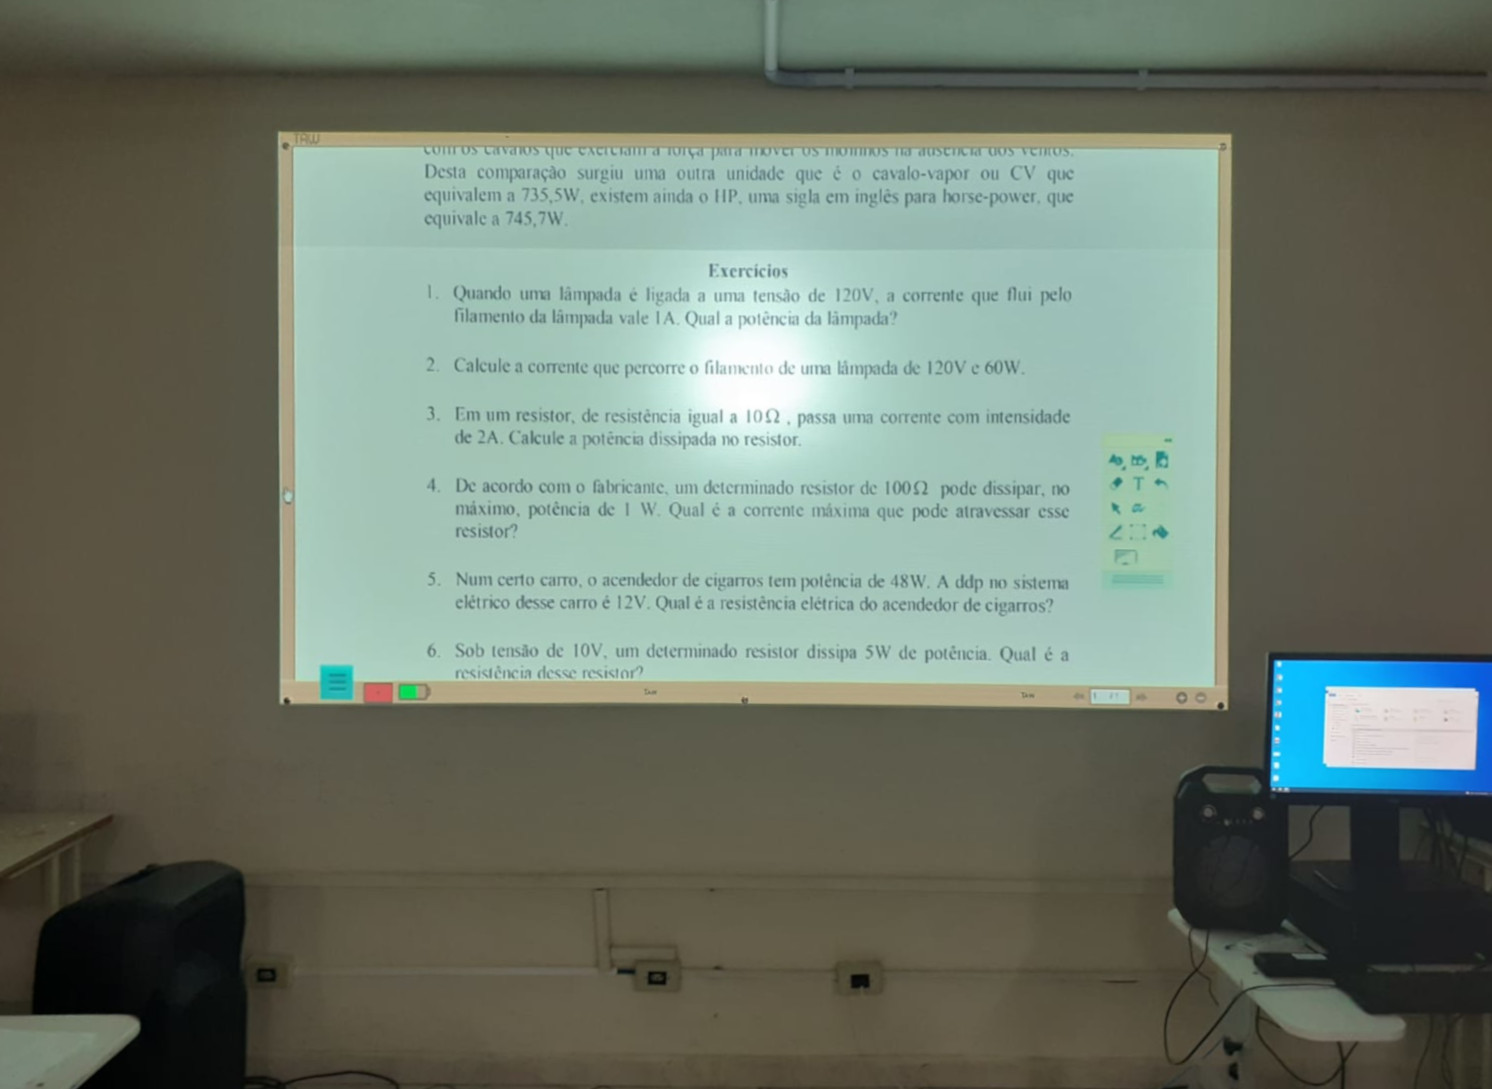
\includegraphics[width=.45\textwidth]{assets/d-lousa.jpeg}
	\legend{Fonte: O autor}
\end{wrapfigure}
Dentre os espaços revitalizados da \ac{GPF}, encontram-se as 11 salas de aulas destinadas ao ensino do \ac{NEM}, cada uma já recebeu 1 Lousa Digital, 1 Desktop e aguardam a instalação, a \autoref{fig:d-lousa} ilustra um exemplo de uso em uma das salas da unidade. A ordem de serviço para a instalação destes recursos já foi liberada o que deve ocorrer nos próximos meses. Além destes recursos todas as salas da unidade ainda contam com 1 Lousa Melamínica Branca, armários e ar-condicionado.
% section Sala de Aula (end)

\section{Laboratório} % (fold)
\label{sec:Laboratório}
As aulas experimentais podem ser conduzidas no Laboratório, preparado para atender as disciplinas de Física, Química e Biologia. Comporta cerca de 40 alunos e é composto por duas grandes bancadas e alguns armários. Há nele matériais para experimentos de cinemática, física dilatação térmica e eletrostática. Geralmente o professor de Física utiliza as salas de aulas para as aulas experimentais, mas se um experimento mais elaborado necessitar de mais recursos, o laboratório é uma boa opção. No semestre em que desenvolveu-se este estágio, o laboratório não estava disponível, pois estava abrigando novos recursos tecnológicos adquiridos pela escola, a previsão de reativação do laboratório está marcada para ocorrer a partir do início do próximo semestre.
% section Laboratório (end)


\section{Auditório} % (fold)
\label{sec:Auditório}
\setlength\intextsep{0pt}
\begin{wrapfigure}[13]{r}{0.5\textwidth}
	\centering
	\caption{Auditório}
	\label{fig:auditorio-01}
	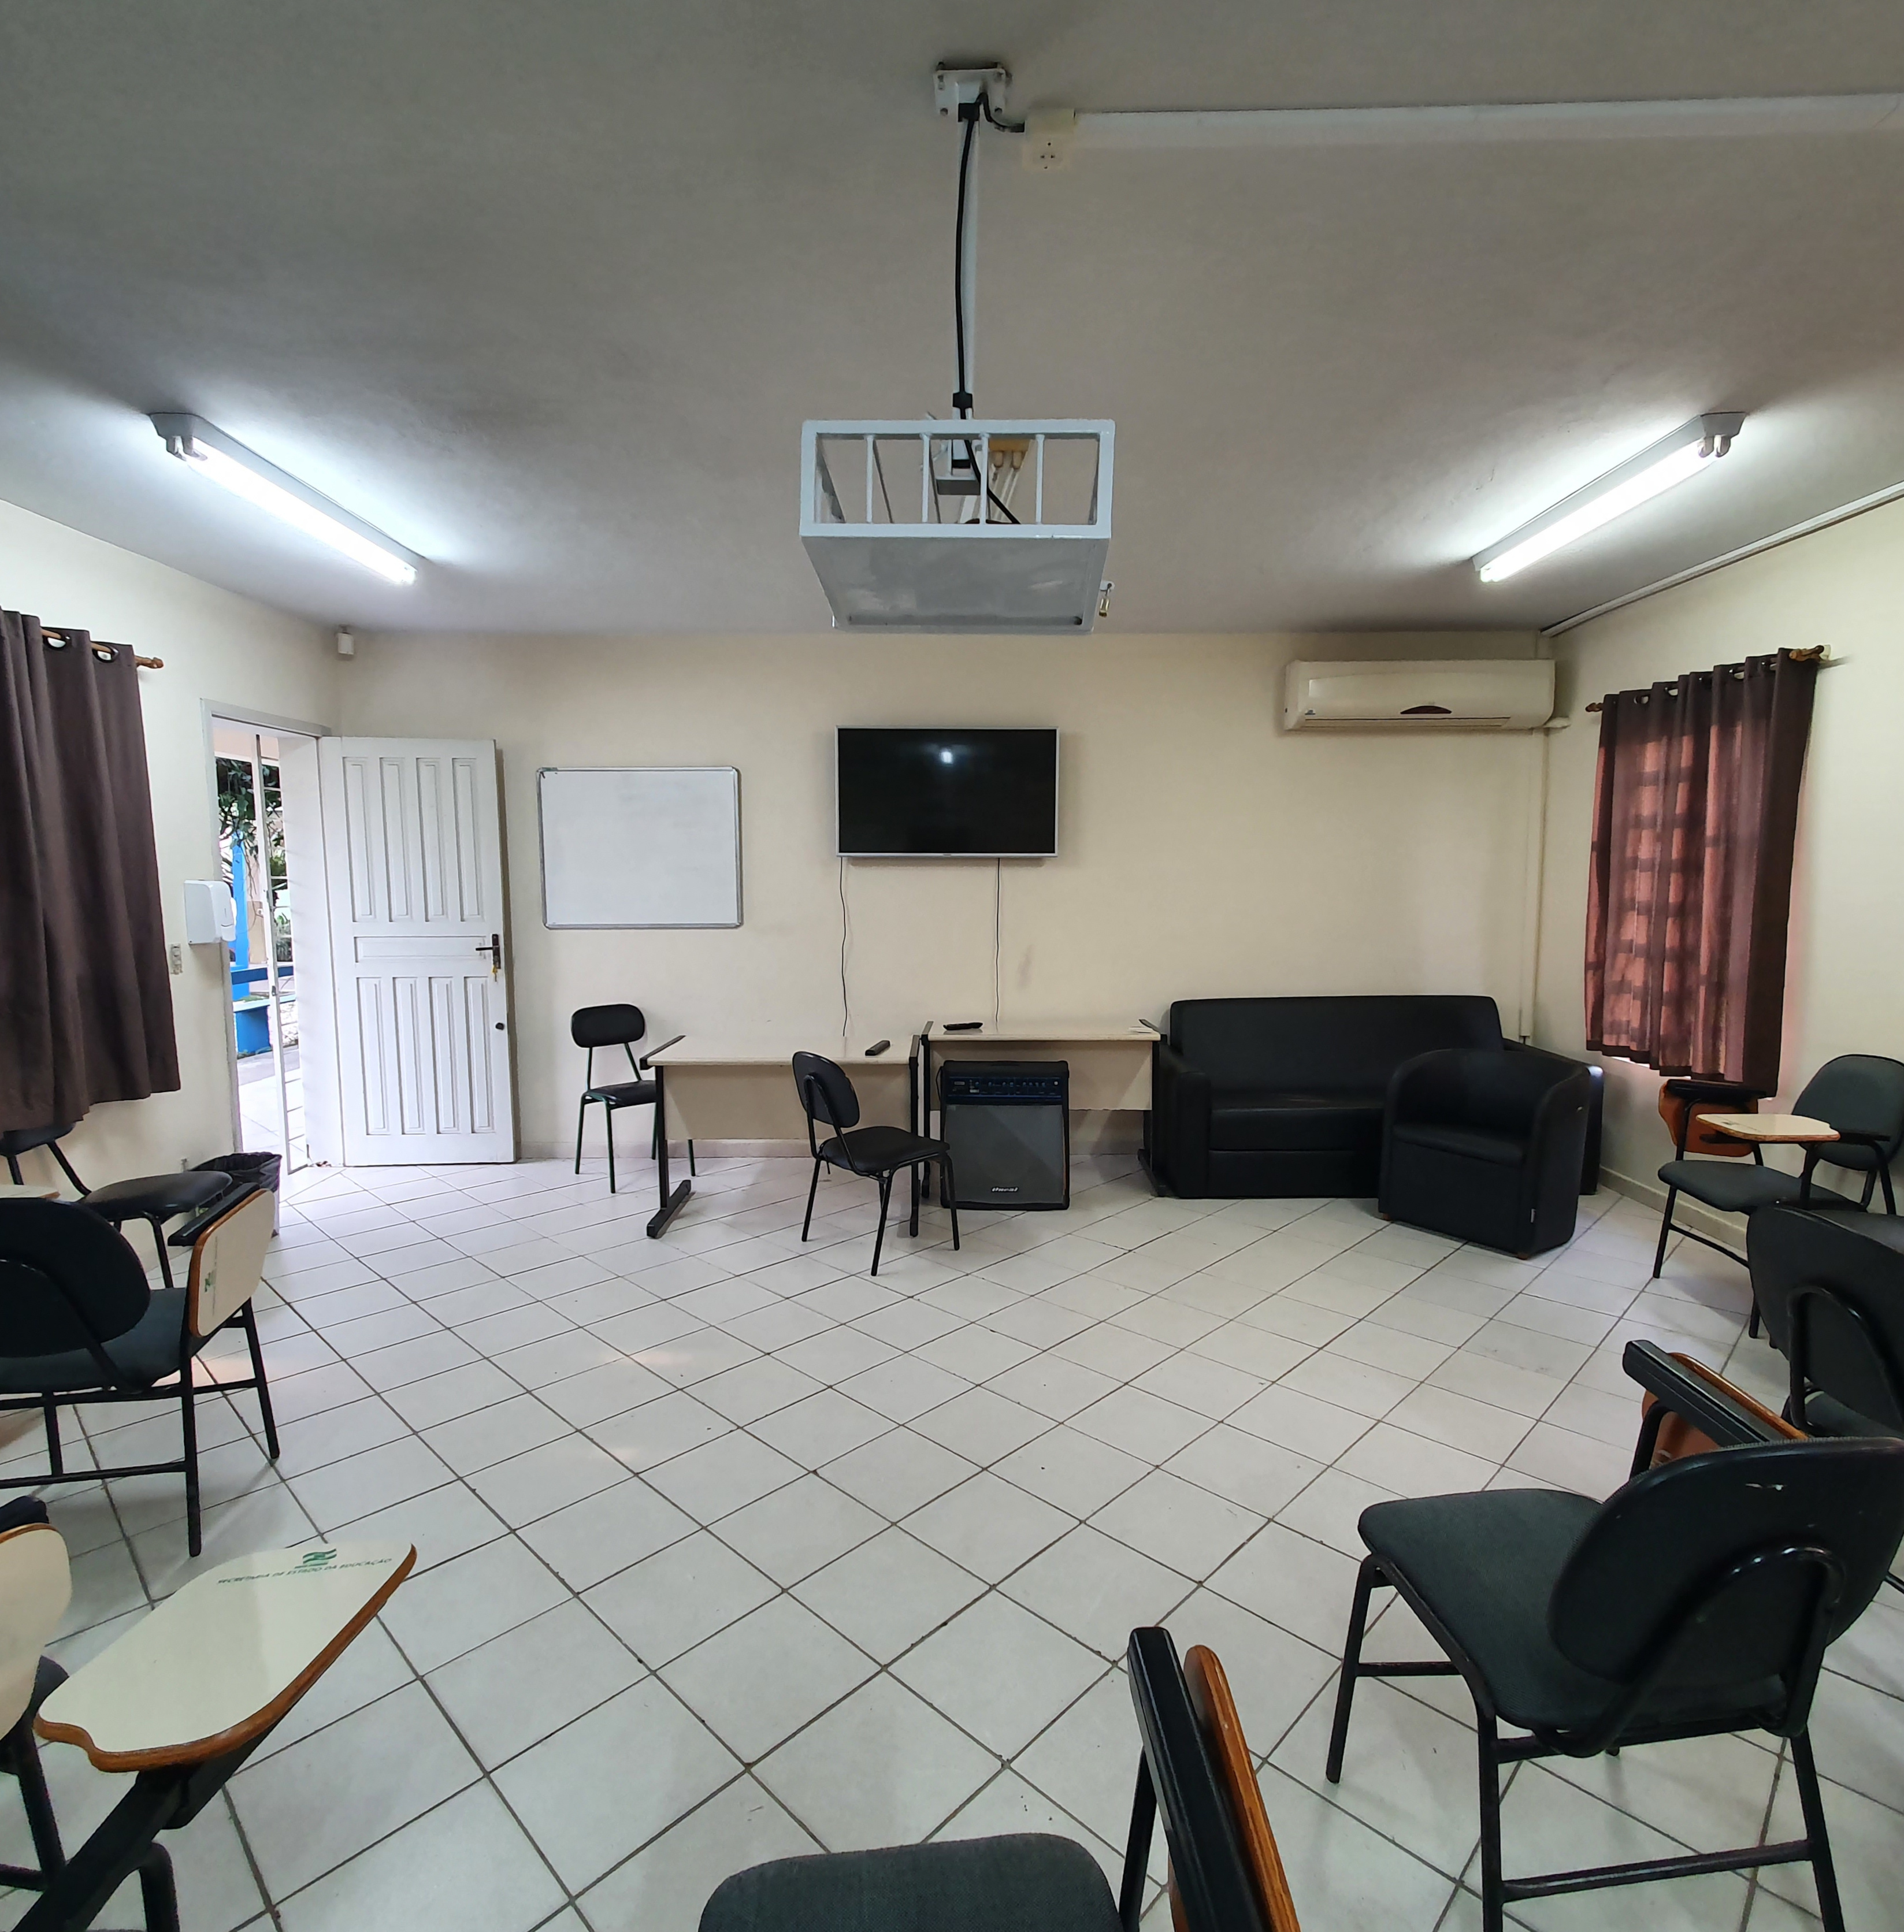
\includegraphics[width=.45\textwidth]{assets/auditorio-01.jpg}
	\legend{Fonte: O autor}
\end{wrapfigure}
O auditório, \autoref{fig:auditorio-01}, tem capacidade para comportar um total de quarenta pessoas e é equipado com um televisor de led $40\inch$, caixa de som amplificada multi-uso, um retroprojetor e ar-condicionado. É frequentemente utilizado para aulas de vídeo, apresentações e também pelo Conselho de Classe.
% section Auditório (end)

\section{Laboratório de Informática} % (fold)
\label{sec:Laboratório de Informática}
Outro espaço revitalizado na \ac{GPF} em 2023, foi o Laboratório de Informática, que recebeu 25 novos computadores. Segundo a direção está funcional porém, a escola aguarda ainda a chegada de um profissional que ficará responsável pelo local, o que deve passar por um processo elaborado pela Secretaria Estadual de Educação no decorrer deste ano, até lá, os professores que desejarem utilizar deste recurso, precisam antes combinar com alguém da equipe técnica/gestora um horário que seja possível para ambos atenderem a turma. Não é permitido o uso do Laboratório apenas pelo professor e sua turma, para evitar extravio de peças e dano aos equipamentos. O local ainda conta com internet banda larga cabeada e wi-fi, uma Lousa Melamínica Branca e um retroprojetor já devidamente instalados.
% section Laboratório de Informática (end)

\section{Biblioteca} % (fold)
\label{sec:Biblioteca}
De todos os ambientes disponíveis para uso pedagógico na unidade, o menos utilizada em aulas de Física foi a Biblioteca, o que não significa que não seja usada em outras disciplinas, em seu acervo encontram-se livros didáticos para todas as disciplinas, livros de literatura nacional e internacional, almanaques, \acp{DVD} educativos, revistas de assuntos dos mais variados e jornais. Possui também uma televisão de $32\inch$ a tubo conectada à uma leitora de \ac{DVD}, mesas e cadeiras o suficiente para comportar uma pequena turma de 10 pessoas tal como pode ser visto na \autoref{fig:biblioteca-01}.
% section Biblioteca (end)

\section{Tablets} % (fold)
\label{sec:Tablets}
A unidade também possui 32 Tablets conectados à internet de 200 Mb e com o sistema operacional Android. Neles, o professor costuma usar o aplicativo \emph{Kahoot} em atividades diferenciadas. Para manter os tablets sempre com a bateria carregadas e prontos para uso, a escola utiliza o gabinete móvel de recarga, como pode ser visto na \autoref{fig:tablets}.
\vspace{15pt}

\begin{figure}[!ht]
	\centering
	\caption{Em (a) imagem do gabinete de recarga dos tablets e em (b) visão interna da Biblioteca da unidade concedente.}
	\label{fig:tablet-biblioteca}
	\begin{subfigure}[b]{.4\textwidth}
		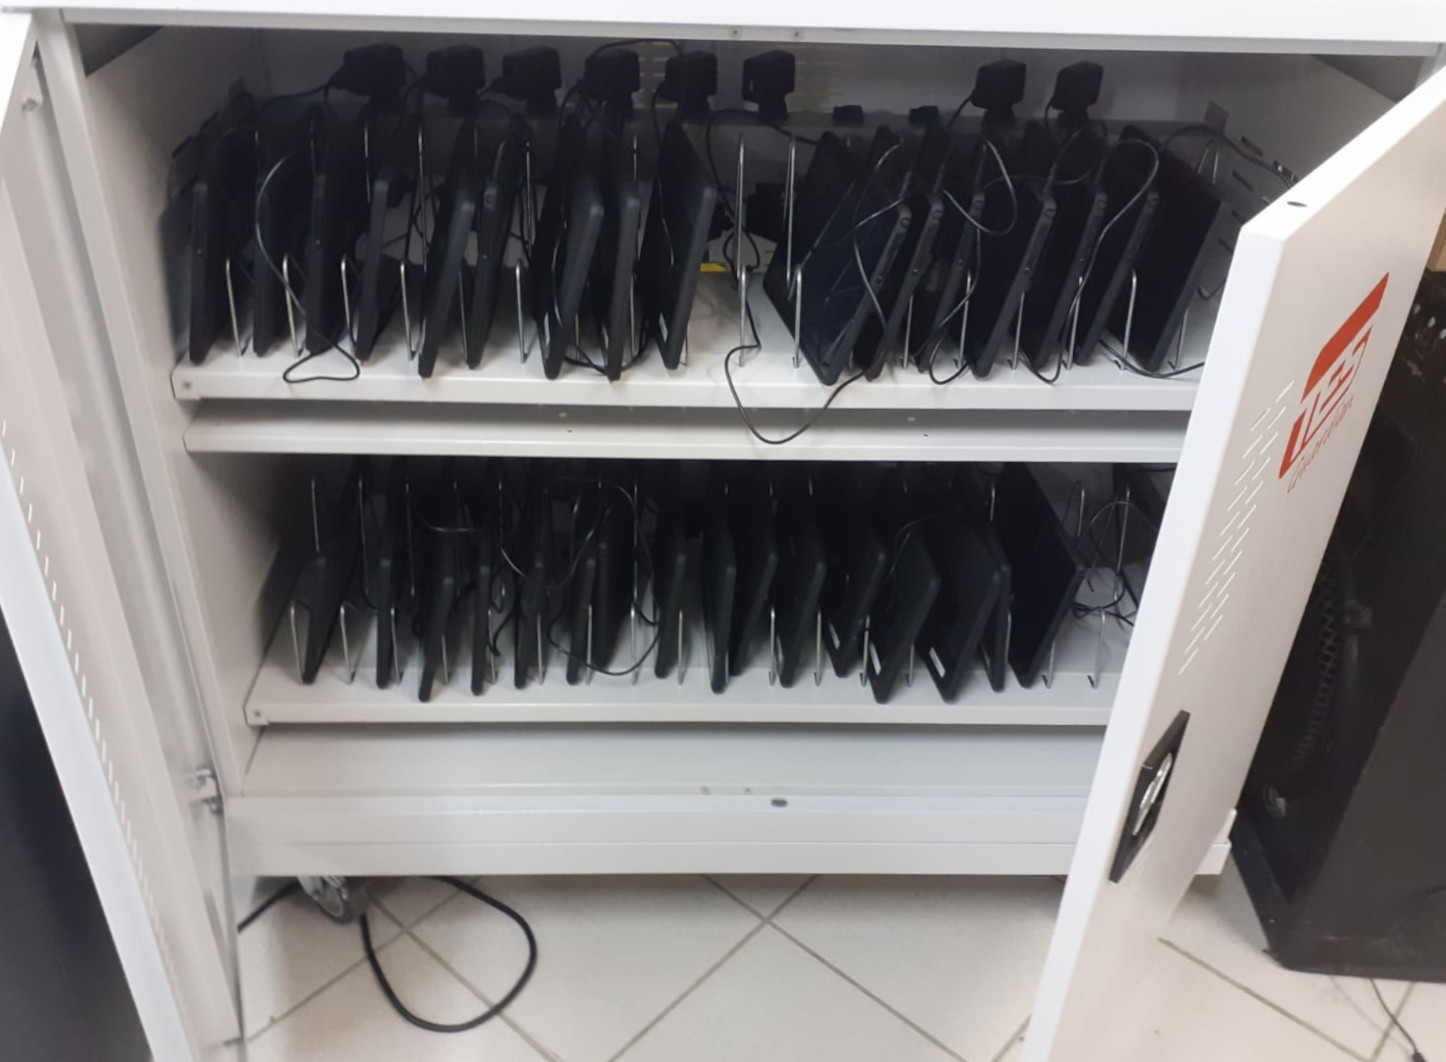
\includegraphics[width=\textwidth]{assets/tablets.jpeg}			
		\caption{Tablets}
		\label{fig:tablets}
	\end{subfigure}
	\hspace{20pt}
	\begin{subfigure}[b]{.4\textwidth}
		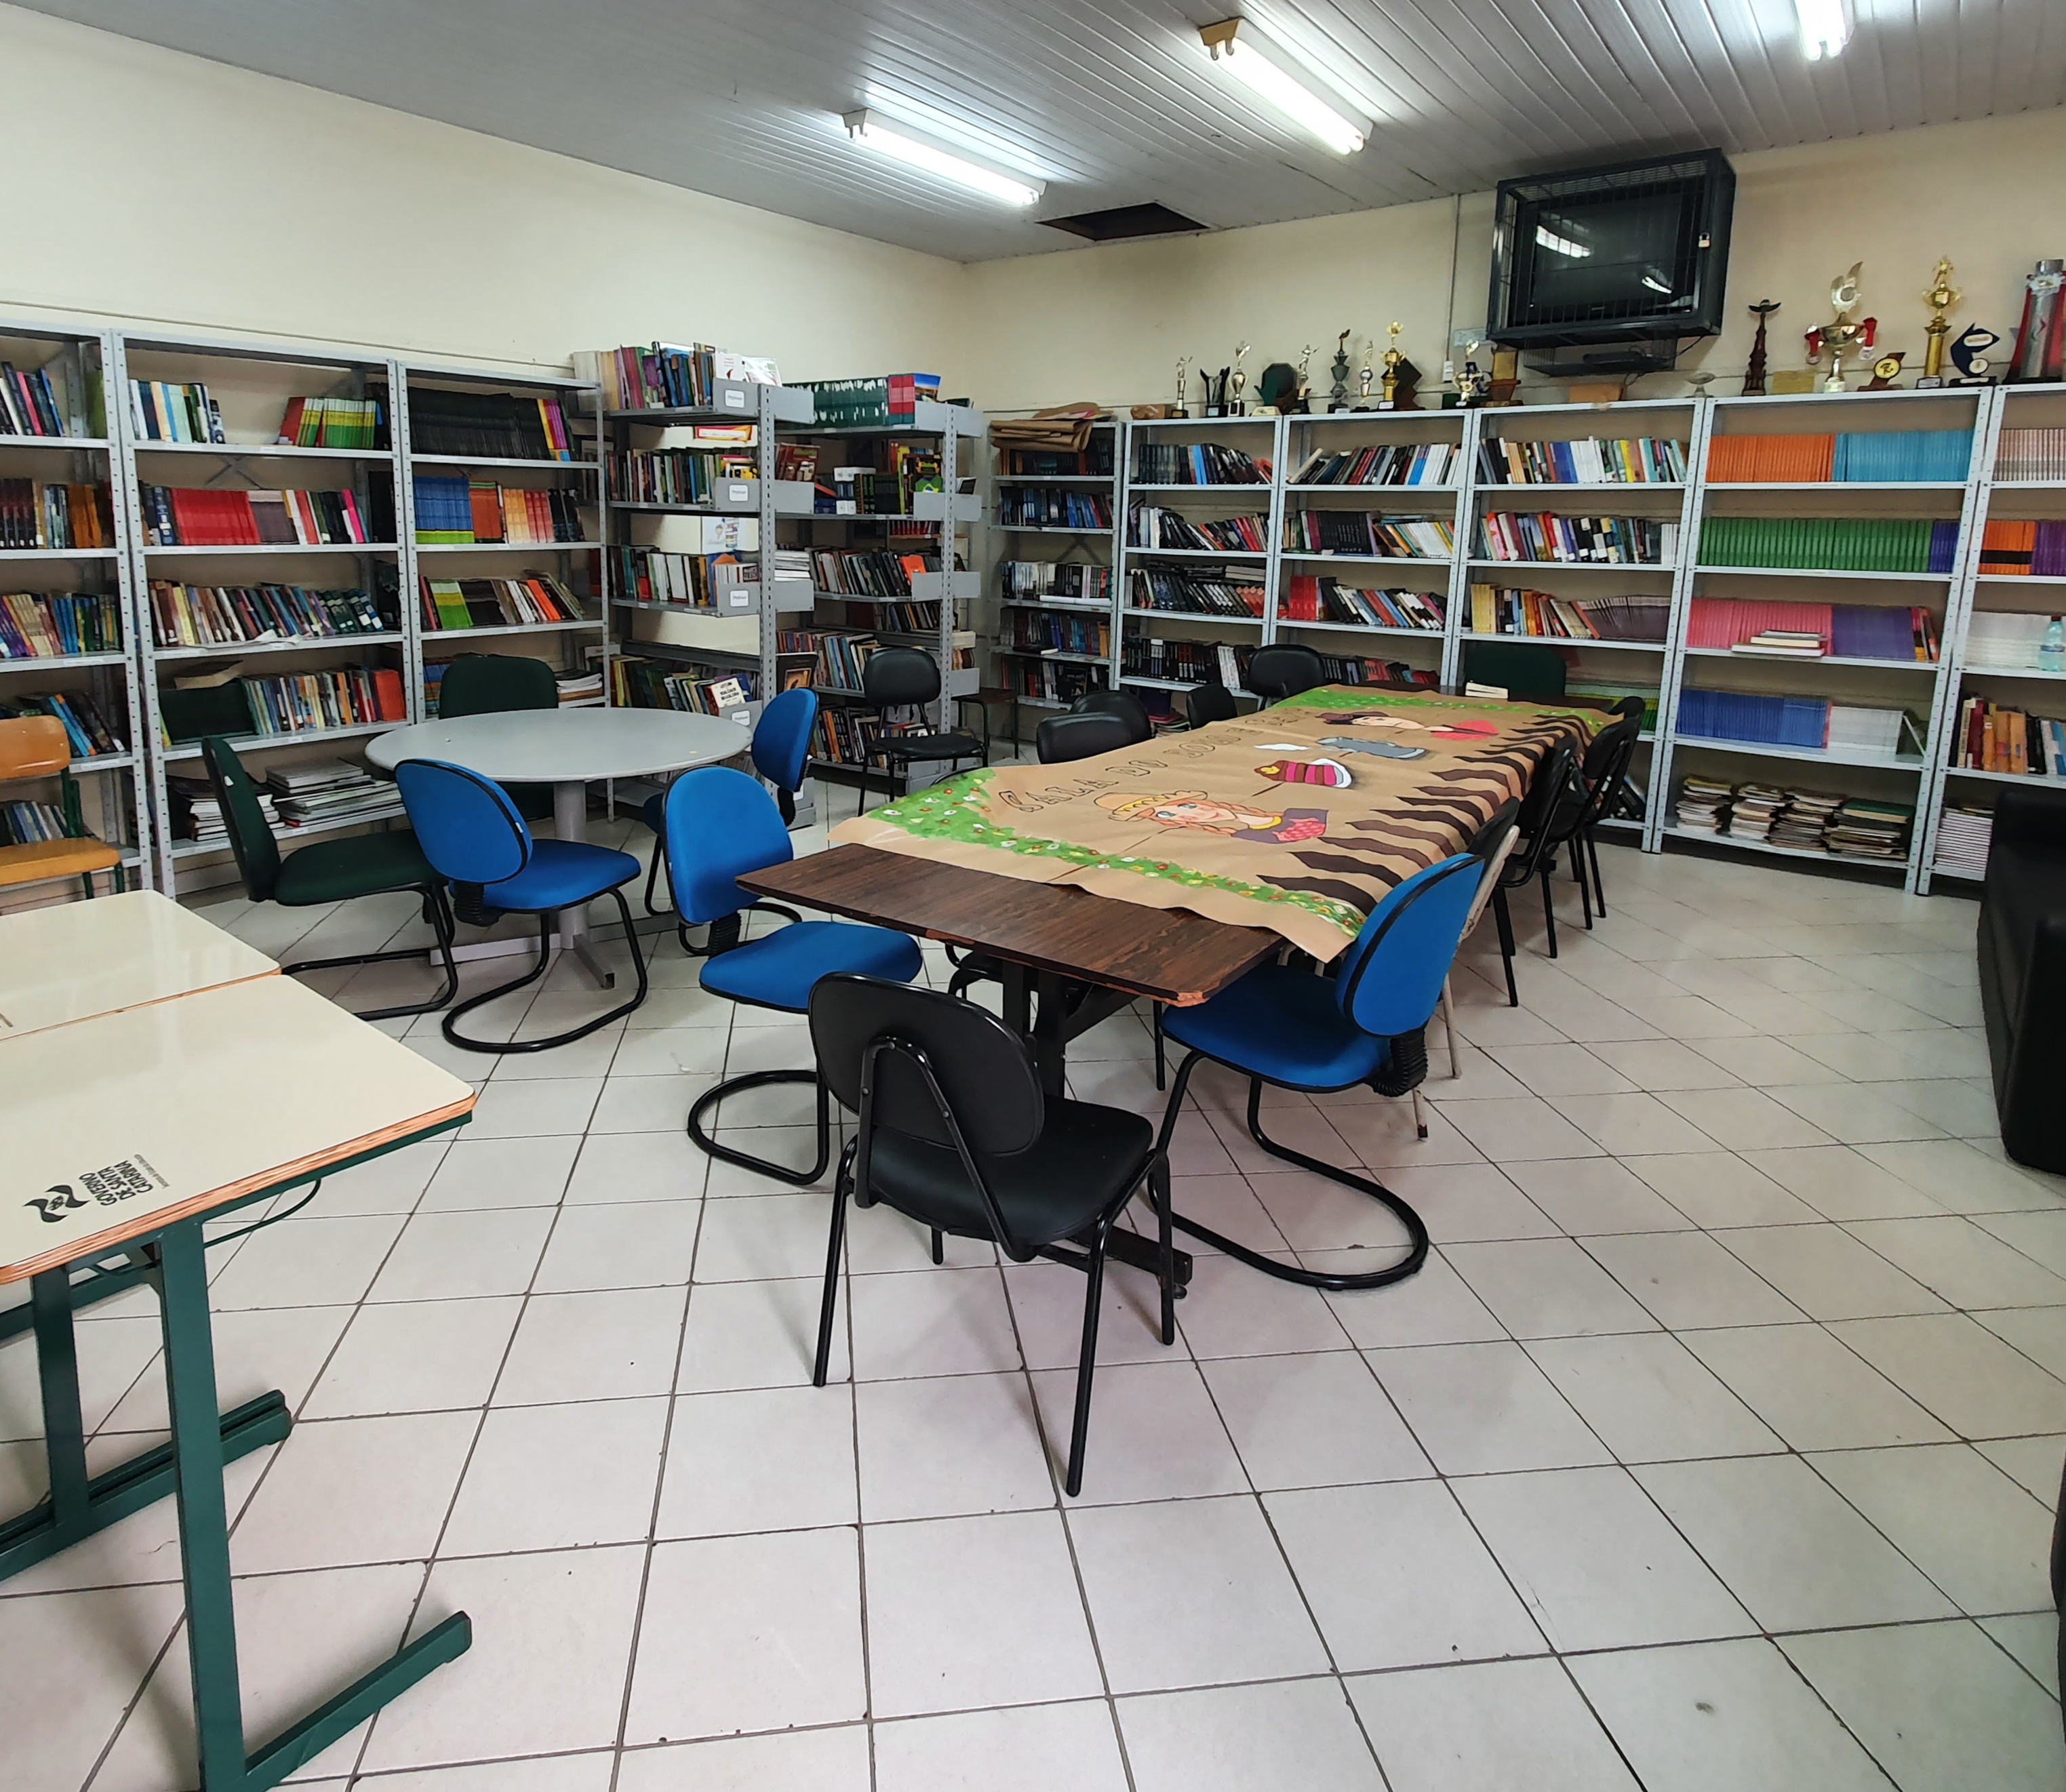
\includegraphics[width=\textwidth]{assets/biblioteca-01.jpg}
		\caption{Biblioteca}
		\label{fig:biblioteca-01}
	\end{subfigure}
	\legend{Fonte: O autor}
\end{figure}

% section Tablets (end)
% chapter Apoio à Docência (end)
